\label{chap:benchmark_results}
Benchmark data sets enable fair comparisons of ranking models over a fixed set of documents and queries. The approach of using fixed benchmark data sets to compare the performance of Information Retrieval systems under equal circumstances has been the standard evaluation methodology in the Information Retrieval field since the release of the Cranfield collection \cite{Cleverdon1966}.\\

This chapter describes benchmark characteristics, e.g. collection size and features, of Learning to Rank benchmark collections and data sets and gives an overview of the performance of baseline algorithms on these collections and data sets.\\

The accuracies of the Learning to Rank methods described in the following sections can only be compared within the benchmark and not between benchmarks for the following reasons:
\begin{enumerate}
\item Differences in feature sets between data sets detract from fair comparison
\item Although the \ac{nDCG} definition is unambiguous, Busa-Fekete et al. \cite{Busa-Fekete2012} found that \ac{nDCG} evaluation tools of benchmark data sets produced different scores
\end{enumerate}

\section{Yahoo! Learning to Rank Challenge}
Yahoo's observation that all existing benchmark data sets were too small to draw reliable conclusions prompted Yahoo to release two internal data sets from Yahoo! search. Data sets used at commercial search engines are many times larger than available benchmark data sets. Yahoo! published a subset of their own commercial training data and launched a Learning to Rank competition based on this data. The Yahoo! Learning to Rank Challenge \cite{Chapelle2011a} is a public Learning to Rank competition which took place from March to May 2010, with the goal to promote the data sets and encourage the research community to develop new Learning to Rank algorithms.\\

The Yahoo! Learning to Rank Challenge consists of two tracks that uses the two data sets respectively: a standard Learning to Rank track and a transfer learning track where the goal was to learn a specialized ranking function that can be used for a small country by leveraging a larger training set of another country. For this experiment, I will only look at the standard Learning to Rank data set, because transfer learning is a separate research area that is not included in this thesis.\\
\begin{table}[!h]
\begin{tabular}{l|lll}
 & Train & Validation & Test \\ 
 \hline
\# of queries & 19,994 & 2,994 & 6,983 \\ 
\# of documents & 473,134 & 71,083 & 165,660 \\ 
\# of features & 519 & 519 & 519 \\ 
\end{tabular}
\caption{Yahoo! Learning to Rank Challenge data set characteristics, as described in the overview paper \cite{Chapelle2011a}}
\label{tab:yahoo_characteristics}
\end{table}\\
Both \ac{nDCG} and \ac{ERR} are measured as performance metrics, but the final standings of the challenge were based on the \ac{ERR} values. Model validation on the Learning to Rank methods participating in the challenge is performed using a train/validation/test-set split following the characteristics shown in Table \ref{tab:yahoo_characteristics}. Competitors could train on the training set and get immediate feedback on their performance on the validation set. The test set performance is used to create the final standings and is only measured after the competition has ended to avoid overfitting on the test set. The large number of documents, queries and features compared to other benchmark data sets makes the Yahoo! Learning to Rank Challenge data set interesting. Yahoo did not provide detailed feature descriptions to prevent competitors to get detailed insight in the characteristics of the Yahoo data collection and features used at Yahoo. Instead high level descriptions of feature categories are provided. The following categories of features are described in the challenge overview paper \cite{Chapelle2011a}:\\
\begin{description}
\item[Web graph]{Quality and popularity metrics of web documents, e.g. PageRank \cite{Page1999}}.
\item[Document statistics]{Basic document statistics such as the number of words and url characteristics.}
\item[Document classifier]{Results of various classifiers on the documents. These classifiers amongst others include: spam, adult, language, main topic, and quality classifiers.}
\item[Query]{Basic query statistics, such as the number of terms, query frequency, and click-through rate.}
\item[Text match]{Textual similarity metrics between query and document. Includes \ac{TF-IDF}, BM25 \cite{Robertson2009} and other metrics for different sections of the document.}
\item[Topical matching]{These features go beyond similarity at word level and compute similarity on topic level. For example by classifying both the document and the query in a large topical taxonomy.}
\item[Click]{Click-based user feedback.}
\item[External references]{Document meta-information such as Delicious\footnote{https://delicious.com/} tags}
\item[Time]{Document age and historical in- and outlink data that might help for time sensitive queries.}
\end{description}

\subsection{Results}
1055 teams send in at least one submission to the Yahoo! Learning to Rank challenge. The top eight participants of the Yahoo! Learning to Rank challenge all used decision trees combined with ensemble methods. The mainly used ensemble method within these top performers is boosting. The combination of boosting with decision tree learners is often called \acf{GBDT}. Figure \ref{fig:yahoo_results} shows the top five participants in the Yahoo! Learning to Rank Challenge in terms of ERR score.  Burges  \cite{Burges2011} created a linear combination ensemble of eight LambdaMART \cite{Burges2010}, two LambdaRank and two Logistic Regression models. Gottschalk and Vogel used a combination of RandomForest models and \ac{GBDT} models. Pavlov and Brunk used a regression based model using the BagBoo \cite{Pavlov2010} ensemble technique, which combines bagging and boosting. Sorokina used a similar combination of bagging and boosting that is called Additive Groves \cite{Sorokina2007}.\\

The challenge overview paper \cite{Chapelle2011a} states as one of the lessons of the challenge that the simple baseline \ac{GBDT} model performed very well with a small performance gap to the complex ensemble submissions at the top of the table.\\

\begin{table}
\begin{tabular}{l|p{6.3cm}|l}
 & Authors & ERR \\
 \hline 
1 & Burges et al. (Microsoft Research) & 0.46861 \\ 
2 & Gottschalk (Activision Blizzard) \& Vogel (Data Mining Solutions) & 0.46786 \\ 
3 & Parakhin (Microsoft) & 0.46695 \\ 
4 & Pavlov \& Brunk (Yandex Labs) & 0.46678 \\ 
5 & Sorokina (Yandex Labs) & 0.46616 \\ 
\end{tabular}
\caption{Final standings of the Yahoo! Learning to Rank Challenge, as presented in the challenge overview paper \cite{Chapelle2011a}}
\label{fig:yahoo_results}
\end{table}

Although the winning \ac{GBDT} models performs very well in terms of \ac{nDCG} their high complexity makes them unsuitable to use in production. The winning models take weeks to train and are very slow during query evaluation. An exception in training time is the BagBoo \cite{Pavlov2010} method used by Pavlov \& Brunk. The bagging component of the BagBoo method enables it to achieve high scalability through parallelism. Pavlov et al. \cite{Pavlov2010} managed to train half a million trees on 200 nodes in 2 hours.

\section{LETOR}
The LETOR benchmark set was first released by Microsoft Research Asia in April 2007 \cite{Liu2007b} to solve the absence of a experimental platform for Learning to Rank at that time. LETOR has been updated several times since: LETOR 2.0 was released at the end of 2007, LETOR 3.0 \cite{Qin2010} in December 2008 and LETOR 4.0 \cite{Qin2013} in July 2009.

\subsection{LETOR 2.0}
LETOR 2.0 consists of three data sets: the OHSUMED data set and two data sets of the on the .gov collection. The OHSUMED collection is a subset of the medical publication database MEDLINE and contains medical publications from 270 journals that were published between 1987 and 1991. The .gov collection is a web crawl obtained in January 2002, which was used for the \ac{TREC} web track in 2003 and 2004.\\

Different query sets exists for the .gov corpus. Those query sets are categorized in the following categories \cite{Craswell2003}:
\begin{description}
\item[topic distillation (TD)]these queries involve finding relevant pages given a broad query. E.g., the query 'cotton industry' which is entered with the aim to find pages that provide information about the cotton industry.
\item[named page finding (NP)]in these queries the user asks for one specific page by name. E.g., the user queries for 'ADA Enforcement' to find the page $http://www.usdoj.gov/crt/ada/enforce.htm$.
\item[home page finding (HP)]these queries are similar to NP queries in that the user is looking for one specific page, but now this specific page is a homepage. E.g., the user queries for 'Tennessee Valley Authority' to find the homepage $http://www.tva.gov$.
\end{description}

LETOR 2.0 only uses the topic distillation queries. Baseline Learning to Rank algorithms evaluated on LETOR 2.0 by the organisation are:
\begin{description}
\item[pairwise]{\leavevmode
	\begin{itemize}
	\item Rank\ac{SVM} \cite{Herbrich1999,Joachims2002}
	\item RankBoost \cite{Freund2003}
	\item \ac{MHR} \cite{Qin2007}
	\item FRank \cite{Tsai2007}
	\end{itemize}}
\item[listwise]{\leavevmode
	\begin{itemize}
	\item ListNet \cite{Cao2007}
	\item AdaRank-MAP \cite{Xu2007}
	\item AdaRank-nDCG \cite{Xu2007}
	\end{itemize}}
\end{description} 

\subsubsection{Results}
\begin{table}[!h]
\begin{tabular}{l|lll}
 & OHSUMED & TD2003 & TD2004 \\
 \hline 
RankBoost & 0.4356 & 0.2851 & 0.4716 \\ 
Rank\acs{SVM} & 0.4411 & 0.3410 & 0.4201 \\ 
FRank & 0.4423 & 0.3357 & 0.4708 \\ 
ListNet & 0.4489 & 0.3743 & 0.4579 \\ 
AdaRank-\acs{MAP} & 0.4385 & 0.1940 & 0.4063 \\ 
AdaRank-\acs{nDCG} & 0.4369 & 0.2702 & 0.3878 \\ 
\acs{MHR} & 0.4423 &  &  \\ 
\end{tabular}
\caption{\acs{nDCG}@10 results of the baseline methods on LETOR 2.0}
\label{tab:letor2.0_results}
\end{table}
Table \ref{tab:letor2.0_results} shows the performance of the baseline methods on the data sets in the LETOR 2.0 collection. ListNet can be regarded as the winner of the comparison as it outperformed the other methods on two of the three data sets and ranked third on the third data set. \acs{MHR} was only evaluated on the OHSUMED data set, on which it performed second best, after ListNet.


\subsection{LETOR 3.0}
The LETOR 3.0 benchmark collection \cite{Qin2010} as released in 2007 contained two data sets: the OHSUMED collection and the .gov collection. Tables \ref{tbl:features_ohsumed} and \ref{tbl:features_gov} in Appendix \ref{chap:appendix_a} provide the descriptions of the features of the OHSUMED and the .gov collections for LETOR 3.0 respectively. Where LETOR 2.0 only used topic distillation (TD) queries on the .gov corpus, LETOR 3.0 also uses named page finding (NP) and home page finding (HP) queries. With query sets available from both the \ac{TREC} 2003 and 2004 conferences there are six query sets in total: TD2003, TD2004, NP2003, NP2004, HP2003 and HP2004. It is noteworthy that the OHSUMED, TD2003 and TD2004 data sets of LETOR 2.0 and LETOR 3.0 are not identical and therefore not comparable due to differences in sampling method.\\

The evaluation metrics used are \ac{nDCG} and \ac{MAP}. The \emph{winning number} metric is defined as the number of other algorithms that it can beat over all of the seven data sets (six .gov sets + OHSUMED). The LETOR organisation implemented and evaluated several well-known Learning to Rank algorithms themselves and in addition gathers and publications and results of new algorithms evaluated on the LETOR benchmark. The baseline Learning to Rank algorithms evaluated by the LETOR team are:
\begin{description}
\item[pointwise]{\leavevmode
	\begin{itemize}
	\item Linear regression
	\end{itemize}}
\item[pairwise]{\leavevmode
	\begin{itemize}
	\item Rank\ac{SVM} \cite{Herbrich1999,Joachims2002}
	\item RankBoost \cite{Freund2003}
	\item FRank \cite{Tsai2007}
	\end{itemize}}
\item[listwise]{\leavevmode
	\begin{itemize}
	\item ListNet \cite{Cao2007}
	\item AdaRank-MAP \cite{Xu2007}
	\item AdaRank-nDCG \cite{Xu2007}
	\item \ac{SVM}$^{MAP}$ \cite{Yue2007} 
	\end{itemize}}
\end{description} 

\subsubsection{Results}
The LETOR paper \cite{Qin2010} describes the performance of the LETOR baseline methods. Figures \ref{fig:ndcg_winning_number} and \ref{fig:map_winning_number} show ListNet to be the best performing baseline in terms of winning number on both \ac{nDCG} and \ac{MAP}. The LETOR website lists\footnote{http://research.microsoft.com/en-us/um/beijing/projects/letor/letor3baseline.aspx} a few algorithms that have since been evaluated on the LETOR benchmark collection.\\

\begin{figure}[!h]
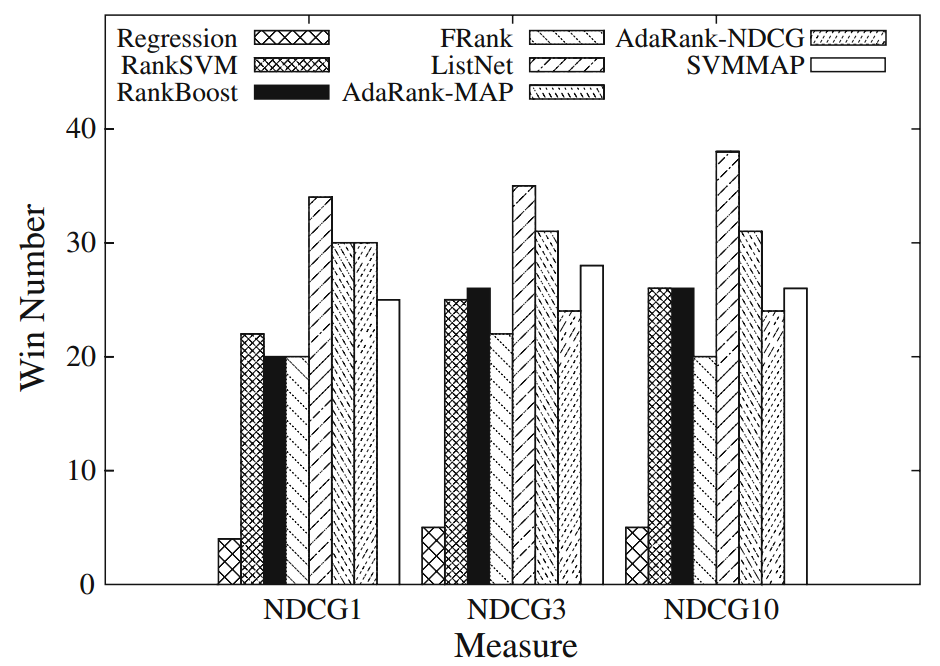
\includegraphics[scale=0.30]{gfx/ndcg_winning_number}
\caption{Comparison of ranking accuracy across the seven data sets in LETOR by \acs{NDCG}, obtained from Qin et al. \cite{Qin2010}}
\label{fig:ndcg_winning_number}
\end{figure}

\begin{figure}[!h]
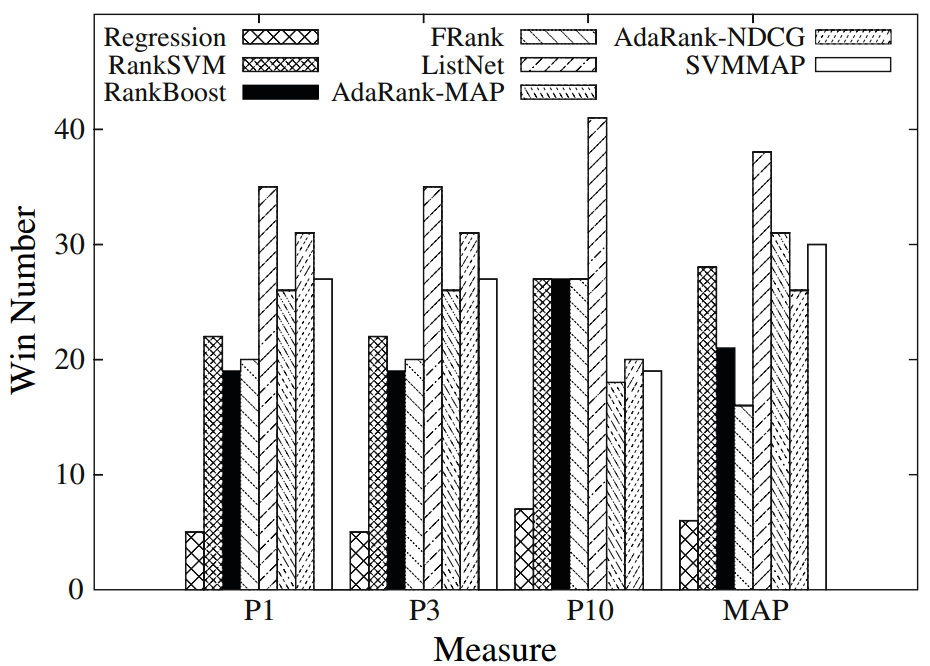
\includegraphics[scale=0.30]{gfx/map_winning_number}
\caption{Comparison across the seven data sets in LETOR by \acs{MAP}, obtained from Qin et al. \cite{Qin2010}}
\label{fig:map_winning_number}
\end{figure}

I will describe the performance of the algorithms that were evaluated by the LETOR team on LETOR 3.0 after publication of the LETOR paper by Qin et al. \cite{Qin2010}, as listed on the LETOR website\footnotemark[2] by comparing their performance with the ListNet baseline. We will consider those methods to be better than ListNet when they beat the ListNet baseline in at least four of the seven data sets in \ac{nDCG} value. Note that this does not necessarily imply that these methods would have scored a higher \ac{nDCG} winning number than ListNet. Table \ref{tbl:LETOR_ListNet} shows the ListNet performance on the seven LETOR data sets in terms of \ac{nDCG}@10 and \ac{MAP}.
\begin{table}[!h]
\begin{tabular}{l|ll}
 & \ac{nDCG}@10 & \ac{MAP} \\ 
 \hline
TD2003 & 0.348 & 0.2753 \\ 
TD2004 & 0.317 & 0.2231 \\ 
NP2003 & 0.801 & 0.6895 \\ 
NP2004 & 0.812 & 0.6720 \\ 
HP2003 & 0.837 & 0.7659 \\ 
HP2004 & 0.784 & 0.6899 \\ 
OHSUMED & 0.441 & 0.4457 \\ 
\end{tabular}
\caption{Performance of ListNet on LETOR 3.0}
\label{tbl:LETOR_ListNet}
\end{table}

Since LETOR is arguably the most well-known benchmark collection in the field, it is conceivable that creators of new Learning to Rank methods evaluate their new method on the LETOR collection to show how well their new method works.

\begin{table}[!h]
\begin{tabular}{l|p{1.2cm}p{1.2cm}p{1.2cm}p{1.4cm}||l}
 & \rotatebox{55}{Ridge Regression} & \rotatebox{55}{Rank\ac{SVM}-Primal} &\rotatebox{55}{Rank\ac{SVM}-Struct} & \rotatebox{55}{SmoothRank} & \rotatebox{55}{ListNet} \\
 \hline
TD2003 & 0.3297 & 0.3571 & 0.3467 & 0.3367 & 0.348 \\ 
TD2004 & 0.2832 & 0.2913 & 0.3090 & 0.3343 & 0.317 \\ 
NP2003 & 0.8025 & 0.7894 & 0.7955 & 0.7986 & 0.801 \\ 
NP2004 & 0.8040 & 0.7950 & 0.7977 & 0.8075 & 0.812 \\ 
HP2003 & 0.8216 & 0.8180 & 0.8162 & 0.8325 & 0.837 \\ 
HP2004 & 0.7188 & 0.7720 & 0.7666 & 0.8221 & 0.784 \\ 
OHSUMED & 0.4436 & 0.4504 & 0.4523 & 0.4568 & 0.441 \\ 
\# winning data sets & 2 & 2 & 1 & 3 & - \\ 
\end{tabular}
\caption{\acs{nDCG}@10 comparison of algorithms recently evaluated on LETOR 3.0 with the ListNet baselines}
\label{tbl:LETOR_recently_added}
\end{table}

\subsection{LETOR 4.0}
The LETOR 4.0 benchmark collection\footnote{http://http://research.microsoft.com/en-us/um/beijing/projects/letor/} consists of the Gov-2 document collection and two query data sets from the Million Query Track at \ac{TREC} 2007 (MQ2007) and \ac{TREC} 2008 (MQ2008). LETOR 4.0 consists of a semi-supervised ranking task, a rank aggregation task and a listwise ranking task next to the supervised ranking task. Table \ref{tab:letor4_characteristics} shows the collection characteristics in number of queries, documents and features for LETOR 4.0. Evaluation on this collection is performed using a five-fold cross-validation, where partitioning of the data into folds was performed beforehand by the creators of the MQ2007 and MQ2008 data sets. Documents in the data set were 

\begin{table}
\begin{tabular}{l|ll}
 Data set & MQ2007 & MQ2008 \\ 
 \hline
 Queries & 1692 & 784 \\ 
 Documents & 69,622 & 15,211 \\
 Features & 46 & 46 \\
\end{tabular}
\caption{Characteristics of the LETOR 4.0 collection}
\label{tab:letor4_characteristics}
\end{table}
\subsubsection{Results}
Rank\ac{SVM}-Struct, ListNet, AdaRank-\ac{nDCG}, AdaRank-\ac{MAP} and RankBoost were used as baseline models on the LETOR 4.0 data set and were implemented and evaluated by the publishers of LETOR 4.0. Table \ref{tab:letor4_baseline_results} shows the performance of those baseline models on the LETOR 4.0 benchmark collection.\\

\begin{table}
\begin{tabular}{l|lll}
Model & Data set & Mean \ac{nDCG} & \ac{nDCG}@10 \\ 
\hline
Rank\ac{SVM}-Struct & MQ2007 & 0.4966 & 0.4439 \\ 
 & MQ2008 & 0.4832 & 0.2279 \\ 
\hline
ListNet & MQ2007 & 0.4988 & 0.4440 \\ 
 & MQ2008 & 0.4914 & 0.2303 \\ 
\hline
AdaRank-\ac{nDCG} & MQ2007 & 0.4914 & 0.4369 \\ 
 & MQ2008 & 0.4950 & 0.2307 \\ 
\hline
AdaRank-\ac{MAP} & MQ2007 & 0.4891 & 0.4335 \\ 
 & MQ2008 & 0.4915 & 0.2288 \\ 
\hline
RankBoost & MQ2007 & 0.5003 & 0.4464 \\ 
 & MQ2008 & 0.4850 & 0.2255 \\ 
\end{tabular}
\caption{Comparison of the LETOR 4.0 baseline models}
\label{tab:letor4_baseline_results}
\end{table}

BoostedTree model \cite{Kocsis2013} showed an \ac{nDCG} of 0.5071 on the MQ2007 data set and thereby beat all baseline models.

\section{Other data sets}
LETOR and the Yahoo! Learning to Rank Challenge data sets are the most used benchmark collections in the field. Several other benchmark collections for the Learning to Rank task have been proposed.

\subsection{MSLR-WEB10/30k}
MSLR-WEB30k and the smaller subset MSLR WEB10k are two large data sets with 30,000 and 10,000 queries respectively. The data was obtained from the Microsoft Bing\footnote{http://www.bing.com/} commercial web search engine. A feature list and feature descriptions are available. The data set only includes features that are commonly used in the research community, as proprietary features were excluded from the data set. Microsoft published these data sets as unofficial successor to LETOR in June 2010, but no baseline evaluations were described by the MSLR-WEB10/30k team. The Microsoft Research website from which the data set is obtainable\footnote{http://research.microsoft.com/en-us/projects/mslr/download.aspx} also offers an evaluation script for \ac{nDCG} and \ac{MAP}. The presence of an official evaluation script enables fair comparison of evaluation results from other researchers comparable.

\subsection{WCL2R}
The WCL2R collection, released by Alc{\^a}ntara et al \cite{Alcantara2010}, contains of two data sets from the Chilean search engine TodoCL\footnote{www.todocl.cl}. Both data sets contain approximately 3 million documents. WCL2R is the only benchmark collection known that provides click-through data on user level. The collection contains 277,095 queries and logs of in total 1,5 million clicks by 16,829 users. The WCL2R paper provides evaluation results for the well-known Rank\ac{SVM} \cite{Herbrich1999,Joachims2002} and RankBoost \cite{Freund2003} algorithms. In addition two ranking methods developed at the same university of the WCL2R paper were evaluated: LAC \cite{Veloso2008} and a ranking algorithm based on \ac{GP} \cite{DeAlmeida2007}. Table \ref{tab:results_WCL2R} shows the performance of those algorithms on the WCL2R collection. No evaluations of other algorithms on the WCL2R collection are known.

\begin{table}[!h]
\begin{tabular}{l|lll|lll}
 &  & FS &  &  & NC &  \\ 
\hline
Algorithm & @1 & @3 & @10 & @1 & @3 & @10 \\ 
\hline
RankSVM & 0.314 & 0.353 & 0.395 & 0.265 & 0.301 & 0.339 \\ 
LAC & 0.296 & 0.360 & 0.403 & 0.244 & 0.266 & 0.315 \\ 
GP & 0.288 & 0.344 & 0.396 & 0.221 & 0.262 & 0.318 \\ 
RankBoost & 0.295 & 0.328 & 0.375 & 0.247 & 0.264 & 0.305 \\ 
\end{tabular}
\caption{\acs{nDCG} results of the baseline methods on the WCL2R collection, obtained from \cite{Alcantara2010}}
\label{tab:results_WCL2R}
\end{table}

\subsection{AOL}
Pass et al. \cite{Pass2006} describe an America Online Learning to Rank data set which they published in 2006. This data set is unique in that it is the only large commercial web search data set that contains user session and user behaviour information. The data set contains 20 million search keywords for over 650,000 users over a three month time period. AOL later realised the publication of the data set to be a mistake, as personally identifiable information turned out to be presented in some of the queries\footnote{http://select.nytimes.com/gst/abstract.html?res=F10612FC345B0C7A8CDDA10894DE404482}. AOL acknowledged the mistake of publishing the data and removed the data from its website. The removal of the data was too late, as the data was already downloadable from several mirror sites\footnote{http://gregsadetsky.com/aol-data/}. This controversial AOL data set is to date still used for Learning to Rank research. No official baseline evaluation is provided by the AOL team.

\subsection{Yandex Internet Mathematics contest}
Russian commercial web search engine Yandex dedicated their yearly Internet Mathematics contest to the task of Learning to Rank in the 2009 edition of the contest. Features (245 in total) are only numbered and their semantics are not revealed, equivalent to the Yahoo! Learning to Rank Challenge. The set is split into a 45\%-training, 10\%-validation, and 45\%-test data. The training set contains 9124 queries, with on average around 100 assessed documents per query. Yandex IMC 2009 has an online leaderboard\footnote{http://imat2009.yandex.ru/en/results} showing the best performing teams in the contest, but it is not traceable which methods each teams used. Pavlov et al. \cite{Pavlov2010} in their paper claim to have won the Yandex Internet Mathematics contest 2009 with their BagBoo method.
